\documentclass[french,12pt]{article}

\usepackage[utf8]{inputenc}
\usepackage[T1]{fontenc}
\usepackage{babel}
\usepackage{hyperref}
\usepackage{lastpage}
\usepackage{graphicx}
\usepackage{listings}
\usepackage{subfig}



\begin{document}
\begin{titlepage}

\newcommand{\HRule}{\rule{\linewidth}{0.5mm}}
\setlength{\topmargin}{0in}
\begin{minipage}{0.4\textwidth}
	\begin{flushleft} \large
		\hspace*{-0.5cm}
		\includegraphics[scale=0.20]{./ressources/logo-unicaen.jpg}
	\end{flushleft}
\end{minipage}
\center
\textsc{\large }\\[0.5cm]
\HRule \\[0.4cm]
{ \huge \bfseries Rapport Aide à la résolution de Kakuro}\\[0.4cm]
\HRule \\[1cm]
\begin{minipage}{\textwidth}
	\begin{flushright} \huge
		\center
		Projet de substitution
	\end{flushright}
\end{minipage}\\[1cm]
\textsc{\large }\\[1cm]
\begin{minipage}{\textwidth}
	\begin{flushright} \large
		\center
		PIGNARD Alexandre - 21701890\\BOCAGE Arthur - 21806332
		\\[1cm]
		L3 Informatique - Promotion 2020-2021
	\end{flushright}
\end{minipage}
\textsc{\large }\\[2cm]
{\large \today}\\[0.5cm]
\vfill
\end{titlepage}

\thispagestyle{empty}
\setcounter{page}{0}
\newpage
\renewcommand{\contentsname}{Table des matières}
\tableofcontents
\newpage


\section{Introduction}
Le \textbf{Kakuro} est un jeu logique semblable aux mots croisés. Le jeu est originaire du Jpaon où sa popularité est immense. Le jeu est similaire aux mots fléchés dans lesquels une même combinaison de chiffres ne peut être utilisé deux fois dans la même grille. Bien que le jeu ne soit parvenu en France que vers les années 2004 et 2005 dans le sillage du sudoku, le jeu reste connu depuis longtemps. \\ \\ Source : Wikipedia \\ \\
Le but de ce projet est de créer un logiciel permettant de fournir une aide à la résolution de grilles de kakuro, il ne s'agit pas de proposer une résolution automatique mais de fournir des outils à un joueur afin qu'il résolve de lui même une grille de jeu. \\\ \\
Pour réaliser ce projet, nous avons choisi le langage Python, permettant de créer un livrable plus rapidement, et nous offrant un large panel de possibilitées pour la création d'interfaces graphiques, nous avons opté pour PyQt5, étant déjà expérimenter avec cette librairie, nous avons fait un gain de temps majeur sur le temps de dévellopement avec ces choix.
\section{Guide d'utilisation du programme}
Afin d'éxecuter le logiciel il faut avoir installé :
\begin{enumerate}
\item[-] Python 3.8 ou +
\item[-] La Librairie Pickle
\item[-] La Librairie PyQt 5
\end{enumerate} 
Pour utiliser notre programme, vous pouvez vous rendre dans le répertoire $Kakuro$\_$Helper$ et lancer la commande :
\begin{lstlisting}[language=bash]
  $ python3 Main.py
\end{lstlisting}

\newpage

\section{Architecture logique de l'application}

\begin{figure}[ht]
  \begin{center}
    \includegraphics[width=\textwidth]{./ressources/diagramme2.png} 
  \end{center}
  \caption{Interactions des fenêtres.}
\end{figure}

\begin{figure}[ht]
  \begin{center}
    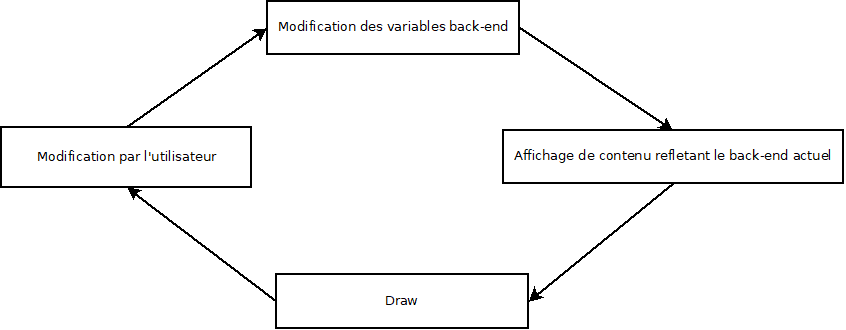
\includegraphics[scale=0.5]{./ressources/diagramme1.png} 
  \end{center}
  \caption{Interactions refresh.}
\end{figure}

\newpage
\section{Conception du programme : Back-end}
Le code présent dans le répertoire back-end constitue le cœur logique du logiciel. Il correspond aux méthodes qui vont permettre de créer un grille, y associer des valeurs à jouer ou  encore une "heat map". Il s'agit du travail en arrière plan que l'utilisateur ne verra pas et qui sera utilisé par la partie front-end pour interagir avec l'utilisateur.
\\ \\ 
Le back-end est constitué de deux sous parties : la partie Logic et les Ressources qui pourront être utilisées. \\ \\
La partie Logic contient les fonctions de calcul des filtres et la gestion des sauvegrdes du logiciel et la partie Ressources contient les ressources nécessaires au bon fonctionnement du back-end,pour l'instant uniquement le  dictionnaire des sommes .

 
\subsection{Logique}
\subsubsection{Grid$\_$Logic: la création de la grille}
Le fichier $Grid$\_$Logic.py$ est le fichier Python qui va permettre de gérer la création des grilles de Kakuro. \\ La grille est générée de façon assez classique : il s'agit de listes dans lesquels on trouve d'autres listes. \\
Dans notre logiciel, une grille classique par défault est constituée de 7 fois 7 cases soit 49 cases, chaque case logique est en fait une liste s'étantant sur 6 éléments . \\

\newpage
Il y a six éléments stockés dans une case : \\
\begin{enumerate}
\item[-] String : Type de Case
\item[-] Int : Case de type "heat" (utilisée pour la heat map qui sera détaillée plus loin)
\item[-] List :Liste des objectifs de la case
\item[-] List :Liste des valeurs possibles de la case
\item[-] List :Liste des valeures Contraintes
\item[-] List :Cases sélectionnées
\end{enumerate}
Ici nous avous voulu tirer parti de la flexibilité que python a à l'égard de la gestion des types en ne créant qu'une seule variable pour grille

\subsubsection{Heat$\_$Mapping$\_$Logic : coloration d'une grille}

Le fichier $Heat$\_$Mapping$\_$Logic.py$ contient les fonctions qui vont nous permettre de réaliser une "heat map". Il s'agit de la coloration de la grille qui va permettre de mettre en avant certaines cases en fonction de leur potentiel. Concrètement, plus une case est intéressante à jouer plus elle sera claire. \\
Pour ce faire, dans le tableau une valeur sera attribuée en fonction du nombre de cases libres dans chaque lignes de la grille. Cette valeur est un poids, plus elle est élevée et plus la case sera colorée sur l'interface graphique.  \\ \\

Le fichier est constitué des fonctions suivantes : \\
\begin{itemize}

\item[]$heat$\_$Mapping$\_$Row$ : elle permet de parcourir les cases via un double for, quand elle trouve des cases libres dans  une ligne elle incrémente le poids. \\

\item[]$heat$\_$Mapping$\_$Column$ : même fonctionnement que la fonction ci-dessus mais parcours dans le sens des colonnes. \\

\item[]$Set$\_$Heat$\_$Mapping$ : permet d'appeller les 2 fonctions, de set le poids de bases et de retourner le Kakuro avec une heat map.\\
\end{itemize}

\subsubsection{Possible$\_$Values$\_$Mapping$\_$Logic : guide du remplissage des cases}
Le fichier $Possible$\_$Values$\_$Mapping$\_$Logic.py$ permet de créer le système de recommandation de coups à jouer. C'est ce qui permet d'afficher dans des cases vides les recommandations de chiffres à placer. \\ \\

Les fonctions $objective$\_$Propagation$\_$Row$ et $objective$\_$Propagation$\_$Row$ permettent de parcourir la grille (verticalement et horizontalement) et permettent d'attribuer à chaque cases jouables des objectif et contraintes de jeu pour le calcul des valeures possibles. \\
Ces deux fonctions sont executées par la methode $set$\_$Objective$\_$Propagation$. \\ \\
Quant à la méthode $findCommonNumberForLenght$, elle permet de créer deux sets constitué des solutions possibles à la résolution d'une case en prenant en compte les objectifs et longueurs de chaque contraintes. \\ \\ Le tout étant appelé dans $set$\_$Possible$\_$Values$\_$Mapping$ retournant un kakuro avec toutes les valeures possibles attribuées à chaque cases. 

\subsubsection{Saving$\_$Logic : la gestion de sauvegardes}
Sans le fichier $Saving$\_$Logic.py$ la sauvegarde et le chargement de Kakuro serait impossible car c'est ce fichier qui permet de les gérer. \\
Le code utilise le module pickle pour ce faire et utilise des fichiers au format $.pkl$, qui est simplement un dump mémoire de l'objet voulut.  \\
Il y a deux méthodes de chargement : $load$\_$Default$\_$Save$ qui va permettre de charger un fichier du nom de "save.pkl". On ne peut pas choisir de fichier en particulier. La deuxième méthode de chargement (très similaire) est $load$\_$Kakuro$\_$From$\_$File$, qui prend en argument le nom d'un fichier et qui l'ouvre. \\
La méthode $push$\_$Save$ permet d'écrire un fichier au format $.pkl$ du nom de $save.pkl$. \\ \\
La méthode $dynamic$\_$Load$ permet de charger un fichier de la façon suivante : \\
\begin{enumerate}
\item[-] Vérifie si un fichier "save" est disponible\\
\item[-] Si aucun fichier n'est trouvé alors un Kakuro dit "basique" est crée (il s'agit d'un Kakuro tout prêt fait). \\
\item[-] En revanche, si un fichier "save" est trouvé, alors on le charge.\\
\end{enumerate}

$get$\_$All$\_$Saves$ permet quand à elle de renvoyer les nom de tous les fichiers présents dans le dossier $Saves$.
\subsection{Ressources}
\subsubsection{Dictionnaire des sommes}

Pendant la création du fichier $Possible$\_$Values$\_$Mapping$\_$Logic$, nous nous sommes heurté à un choix, chercher et résoudre les valeures possibles au cas par cas, au besoin, ou créer un fichier contenant toutes les solutions possibles et le loader dans au chargement du programme et au vu des gains de temps; se fut la solution adoptée.\\

Le fichiers $Sums.pkl$ est donc un dictionnaires python de toutes les nombres pouvants être créer avec des chiffres de 1 à 9 sans redondance, pour ca génération nous sommes restés sur une approche naive, mais fonctionnant, étant pas plus neccéssaire dans le programme nous n'avons pas chercher à multi- process/threader les calculs.





\newpage
\section{Conception du programme : Front-end}
\subsection{Fenêtres}
Dans notre logiciel, le front-end sert d'interface homme-machine afin de proposer une grille simple et de permettre à l'utilisateur d'interagir avec cette dernière via des boutons notamment. \\ \\
L'interface graphique a été réalisée grâce à la librairie $PyQt5$. Cette dernière est divisée en plusieurs fenêtres ,constituées de widgets, que l'on appellera windows, de leur nom en anglais et dans les fichiers et qui permettront d'exécuter des tâches spécifiques. \\ \\
Voici la liste : \\

\begin{enumerate}
	\item[-] Une fenêtre d'accueil permettant de sélectionner une grille  \\
	\item[-] Une fenêtre de jeu permettant d'avoir accès aux options d'aide à la 				résolution de la grille de Kakuro que l'on aura sélectionné. \\
	\item[-] Une fenêtre de création de grille qui permettra de créer et sauvegarder sa 		propre grille de Kakuro. \\
	Enfin, c'est dans la partie $Front$\_$End$ que l'on trouve les dossiers de 					sauvegardes, à savoir $Save$ et $Save$\_$Creator$\_$Result$. \\
\end{enumerate}

Pour ce qui est du style de l'interface graphique nous avons opté pour un design simple et sombre (pour préserver le confort des yeux) qui permet de se concentrer sur la grille et les fonctionnalités proposées. On a donc une palette de couleurs allant du gris foncé au gris clair et du orange pastel pour la heat map.
\newpage
\subsubsection{Main$\_$Window : La base de L'UI}

$Main$\_$Window.py$ est le fichier qui va permettre d'initialiser la fenêtre principale qui contiendra toutes les variables importantes du côté back-end pour la session actuelle et hébergera aussi la logique de navigation entre chaque fenêtre, en effet ,sous PyQt5, le changement dynamique du contenu d'une fenêtre n'est pas supporté avec l'achitecture de base, c'est en initialisant un widget "Central" qu'on viendra override, puis ré-affchier que nous sommes arrivés à une interface dynamiqe. \\
\begin{enumerate}
	\item[-] $\_$init$\_$ 
	\item[-] startSolverWindow  
	\item[-] startCreatorWindow 
	\item[-] startLoaderWindow \\
\end{enumerate}
Voici les détails de ces méthodes : \\ \\
La méthode $\_$init$\_$ permet de paramétrer l'interface graphique et d'instancier les variables back-end. On y trouves les paramètres les plus importants comme la taille de la fenêtre, les kakuros logiques,le dictionnaire des sommes, les paramètres de styles généraux ainsi que le premièr apel à méthode d'instanciation de la fenêtre Loader, qui sera le point de départ pour l'utilisateur. \\ \\

$startSolverWindow$, $startCreatorWindow$ et $startLoaderWindow$, comme leur nom l'indique clairement, permettent de d'instancier les widgets des fenêtres de résolution de grilles, de création de grilles ainsi que la fenêtre de choix de grille et d'override le central widget avec le contenu venant d'être créer. \\ \\

Le fichier $Main$\_$Window.py$ est donc la base de l'interface graphique, nous allons maintenant détailler les trois autres window ainsi que les widgets qu'elles utilisent. 




\subsubsection{Solver$\_$Window : la fenêtre principale}

Si l'on ne devait garder qu'une seule fenêtre pour ce logiciel, ce serait evidemment la fenêtre $Solver$\_$Window$. En effet il s'agit de la fenêtre centrale de l'application, celle qui propose les outils d'aide à la résolution de grilles de Kakuro. \\
L'affichage de la fenêtre est simple : en tête un menu permettant de choisir ou non l'affichage de la heat map et/ou des valeurs possible ainsi que la possibilité de charger un autre Kakuro et de se rendre sur la page de création de grilles. \\ \\

Pour ce qui est du code au sein de $Solver$\_$Window.py$, il est agencé de la manière suivante : \\ 
\begin{itemize}
	\item[-] Un constructeur 
	\item[-] Une fonction d'initialisation de la fenêtre qui appelle les widgets 				nécessaires
	\item[-] Une méthode $createMenuLayout$ qui permet de créer le menu de sélection de filtres et de navigation
	\item[-] Ainsi que la plus grosse méthode : $createKakuroSolverLayout$ qui permet de créer la grille centrale. \\
\end{itemize}

$createKakuroSolverLayout$ est la méthode qui permet l'affichage de la grille au milieu de la fenêtre et qui permet d'appeler les fonctions d'aide fournies par le back-end. \\
Elle permet d'afficher la grille, d'afficher la heat map et de fournir les valeurs possibles dans les cases à jouer. Cette méthode contient aussi les styles de la grille et de la heat map. \\
Pour cette dernière nous avons utilisé le format $rgba$ pour la palette graphique, ce dernière nous permet de gérer les traditionnelles valeurs rouge, vert, bleu mais aussi de gérer l'opacité des teintes, ce dernier paramètre est particulièrement utile lors de l'utilisation de la heat map car on peut profiter du poids de chaque case pour adapter l'opacité de la couleur et donc l'intensité de la heat map. \\ 

\newpage

\subsubsection{Loader$\_$Window : page de chargement de grilles}

Le fichier $Loader$\_$Window$ correspond à la page de chargement de grilles, cette page est une fenêtre très simple permettant de sélectionner la grille de Kakuro souhaitée : celle par défaut qui sert de démonstration au logiciel ou bien un Kakuro que l'on aura sauvegardé. \\ \\
La window est simplement constituée d'une boite "box" dans laquelle se trouve un bouton du nom du fichier à charger. Celui-ci dépend de ce que la fonction $createSelectionMenu$ va renvoyer. \\
En effet, celle-ci va parcourir les sauvegardes et créer des boutons en fonctions de celles-ci. Si aucune sauvegarde n'est trouvée alors un bouton ramenant vers la grille de base est crée. 
Une fois cela fait, lorsque l'on clique sur le bouton, la méthode $loadDefaultKakuro$ s'exécute et charge le Kakuro de base.

\subsubsection{Creator$\_$Window}

Parlons à présent du fichier $Creator$\_$Window.py$. Son nom l'indique : il sert à créer la fenêtre d'édition de grille ainsi que la sauvegarde de la grille créée. C'est une fenêtre importante car elle permet à l'utilisateur de créer ses propres grilles de Kakuro afin de s'aider sur les exemples concrets. \\ \\
La fenêtre se présente de la façon suivante : 

\begin{enumerate}
	\item[-] Une grille de bouton servant à créer le Kakuro (des flèches permettent 			d'alterner entre case non jouable, jouable, ou case d'instructions).
	\item[-] Le choix de la dimension de la grille
	\item[-] Deux boutons : un vers la fenêtre d'aide à la résolutions de grilles et un 		autre permettant de sauvegarder la grille crée. \\
\end{enumerate}
\newpage 

Voici les fonctions présentes dans le fichier $Creator$\_$Window.py$ \\
Il y en a 5 : \\

\begin{enumerate}
	\item[-] Un constructeur qui permet de définir les paramètres de base de la fenêtre.
	\item[-] Une fonction $init$\_$UI$ qui permet de créer l'intérieur de la fenêtre : 			styles, création de $VBox$, $layouts$ ainsi que l'affichage de la fenêtre
	\item[-] $create$\_$meneu$\_$layout$ qui permet de créer le menu du bas.
	\item[-] $update$\_$creator$\_$kakuro$\_$dimensions$ qui gère le changement de taille 		de la grille
	\item[-] $create$\_$kakuro$\_$creator$\_$layout$ gère quant à elle la création de la grille d'édition (grâce au widget $Morphing$\_$Label$, détaillé plus loin).
\end{enumerate}
\newpage 



\subsection{Widgets Personnalisés}
Dans cette dernière partie dédiée au code source, nous allons aborder les widgets que nous avons du créer pour par les windows du front-end. \\
Les widgets permettent de créer des portions de code plus facilement implémentable dans les fenêtres, ce qui rend le code moins lourd, plus lisible et facilite la maintenance de l'application. \\ \\
 La liste: \\

\begin{enumerate}
	\item[-] $ContentButton$
	\item[-] $DividedLabel$
	\item[-] $LoaderButton$
	\item[-] $MorphingLabel$ \\
\end{enumerate}

\subsubsection{Content$\_$Button$\_$Widget}
Ce widget est utilisé pour les boutons au sein des cases servant à selectionner des valeurs à jouer. Il permet aussi de créer les contraintes. C'est le widget qui gère le contenu des cases au sein des grilles et est donc un widget particulièrement important. \\ \\
Dans le fonctionnent, la méthode $change$\_$Content$ gère tout ,si un ContentButon est séléctionné alors la valeur ne peut pas être présente dans la ligne, on va donc utiliser les méthodes de propagation qui vont permettre de retirer la valeur dans toute la ligne afin qu'elle ne soit jouable qu'une fois et rahoute le boutons à liste des boutons préssés, quand l'utilisateur désélectionne le bouton, l'inverse se passe , propagation de la libération de contraintes, on retire le bouton actuel de la liste des boutons préssés. 
\\


\newpage
\subsubsection{Divided$\_$Label$\_$Widget}

Ce widget sert à créer au miaximum neuf ContentButtons au sein d'une case représentant au les coups possibles et seront affichés ou non en fonction des lignes des contraintes de jeu imposées par l'utilisateur . \\
Ce widget est court, relativement simple et ne contient que peu de logique,juste le calcul de l'ensemble des valeures possibles moins celui des contraintes et une recherche dans la liste des valeures préssées si des boutons ont étaient là aussi sélectionnés par l'utilisateur. 

\subsubsection{Loader$\_$Button$\_$Widget}

Les $LoaderButtons$ sont générés dans la fenêtre $Loader$\_$Window.py$ et servent à charger un fichier au format $.pkl$ dans le programme pour l'utiliser dans le solver.Utiliser de pair avec la fonction $get_All_Saves$ pour créer un LoaderButton pour chaque fichier de sauvegarde trouvés. \\


\subsubsection{Morphing$\_$Label}

Le dernier widget est $Morphing$\_$Label$, il représente une case du créateur de kakuro,elle permet d'alterner entre case jouable, non jouable et d'instruction dans la grille de la fenêtre de création. \\
Le constructeur permet de spécifier les paramètres des cases : taille, contenu et type.  \\
La méthode $updateCaseType$ reliée au deux boutons dans la barre de sélection  permet de changer le type de la case dans le kakuro Créateur back-end et de re-dessiner la kakuro créateur mis-à jour .

\subsection{Dossiers de sauvegardes}

Pour ce qui est des dossiers de sauvegarde, il y en a deux:  le dossier $Save$ qui contient les sauvegardes seront accèssible par le programme en lecture et le dossier $Save$\_$Creator$\_$Result$ qui contient les nouvelles sauvegardes crées par l'interface de créateur de kakuros. \\
Pour utiliser une sauvegarde crée il faut donc la déplacer du dossier \\ $Save$\_$Creator$\_$Result$ vers $Save$ et éventuellement la renommer.

\section{Le logiciel dans son ensemble}

Voici un exemple d'utilisation du logiciel : si un utilisateur veut résoudre une grille de Kakuro il peut lancer le logiciel et entrer dans l'éditeur de grilles, après avoir spécifié la taille de sa grille il peut commencer à l'éditer. Une fois cela fait il peut enregistrer sa grille et mettre la sauvegarde au format $.pkl$ dans le dossier $Save$. \\ Une fois cela fait il peut désormais utiliser le logiciel pour charger son Kakuro et l'utiliser pour s'aider à résoudre sa grille grâce à la heat map et aux indications de coups à jouer. 

\section{Améliorations possibles}

Le logiciel n'est pas parfait et certaines fonctionnalité n'ont pas été implémentées par manque de temps. \\
Voici une liste de fonctionnalités qui auraient trouvés leur place au sein de ce logiciel : \\

\begin{enumerate}
	\item[-] Rajout d'options dans le système de sauvegarde
	\item[-] Une résolution automatique d'une grille de Kakuro afin de se corriger (sort du thème donc non implémenter)
	\item[-] Amélioration du système de recommandation et nouveaux filtres
	\item[-] Amélioration de l'interface graphique
\end{enumerate}

\newpage
\section{Annexes}


\begin{figure}[ht]
  \begin{center}
    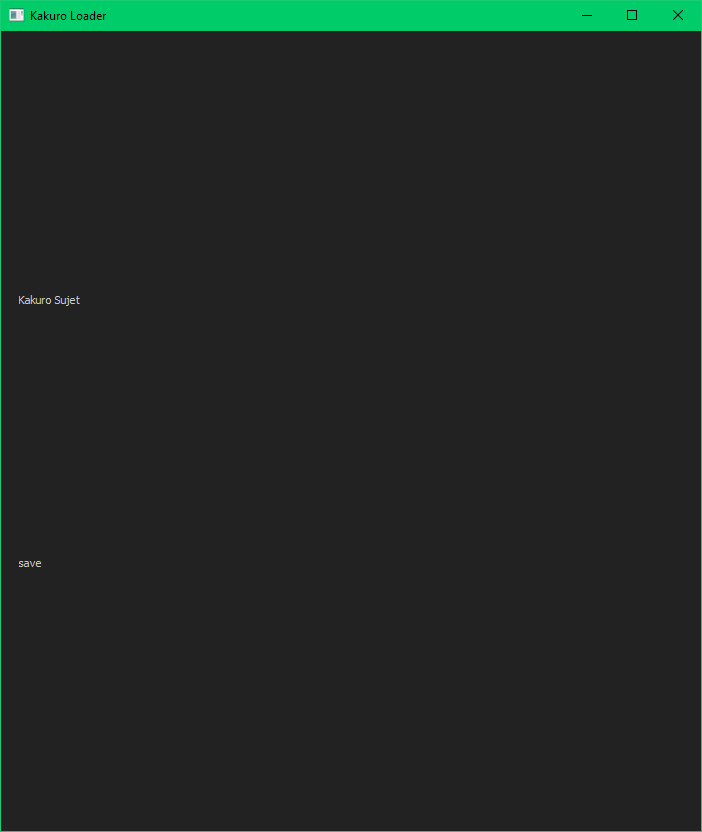
\includegraphics[width=\textwidth]{./ressources/acceuil.png} 
  \end{center}
  \caption{La fenêtre d'accueil.}
\end{figure}

\begin{figure}[ht]
  \begin{center}
    \includegraphics[width=\textwidth]{./ressources/helperSide.png} 
  \end{center}
  \caption{La fenêtre d'aide à la résolution de grilles.}
\end{figure}

\begin{figure}[ht]
  \begin{center}
    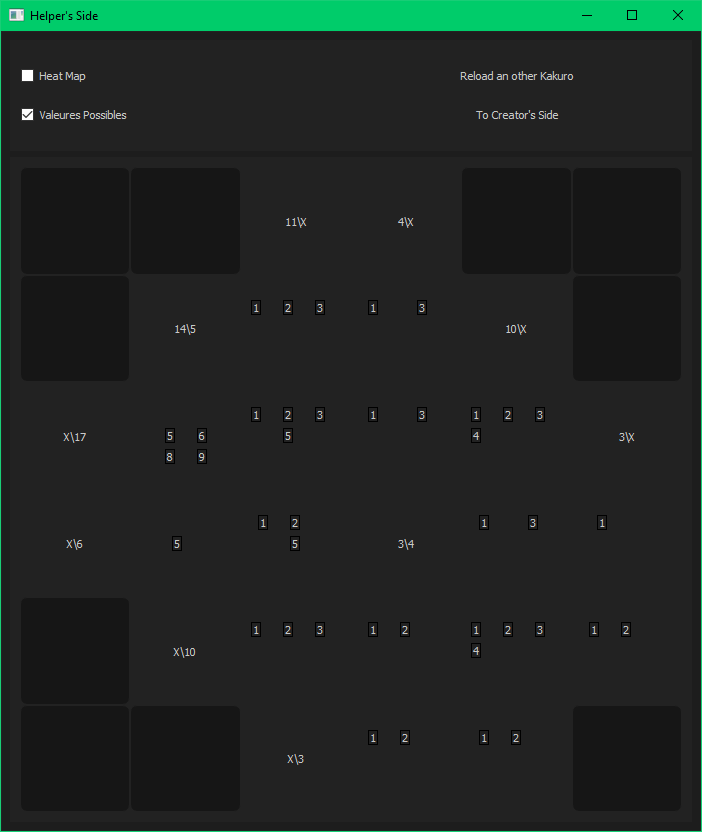
\includegraphics[width=\textwidth]{./ressources/valPoss.png} 
  \end{center}
  \caption{L'affichage des valeurs à jouer.}
\end{figure}

\begin{figure}[ht]
  \begin{center}
    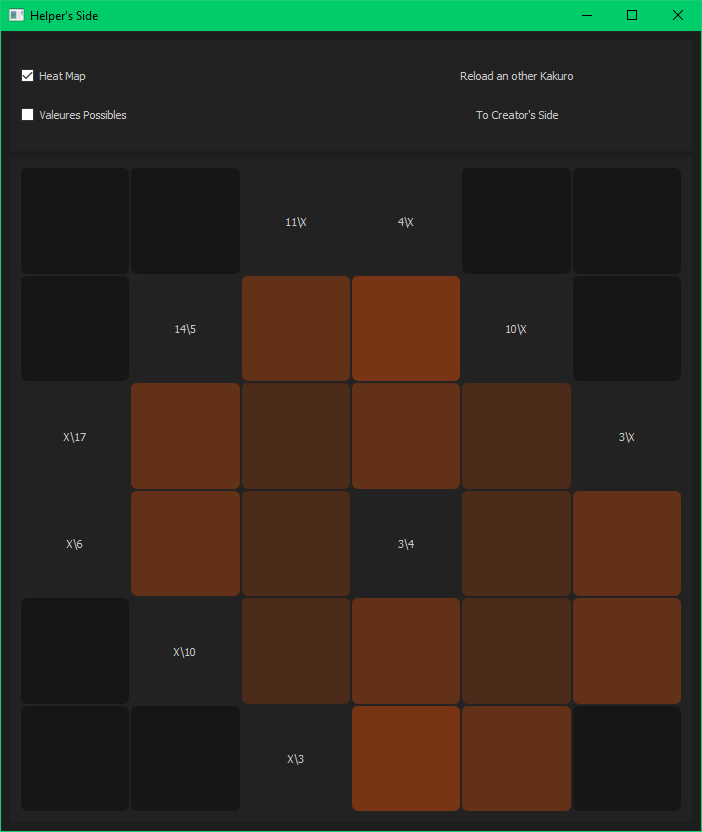
\includegraphics[width=\textwidth]{./ressources/heatmap.png} 
  \end{center}
  \caption{L'affichage de la heat map.}
\end{figure}

\begin{figure}[ht]
  \begin{center}
    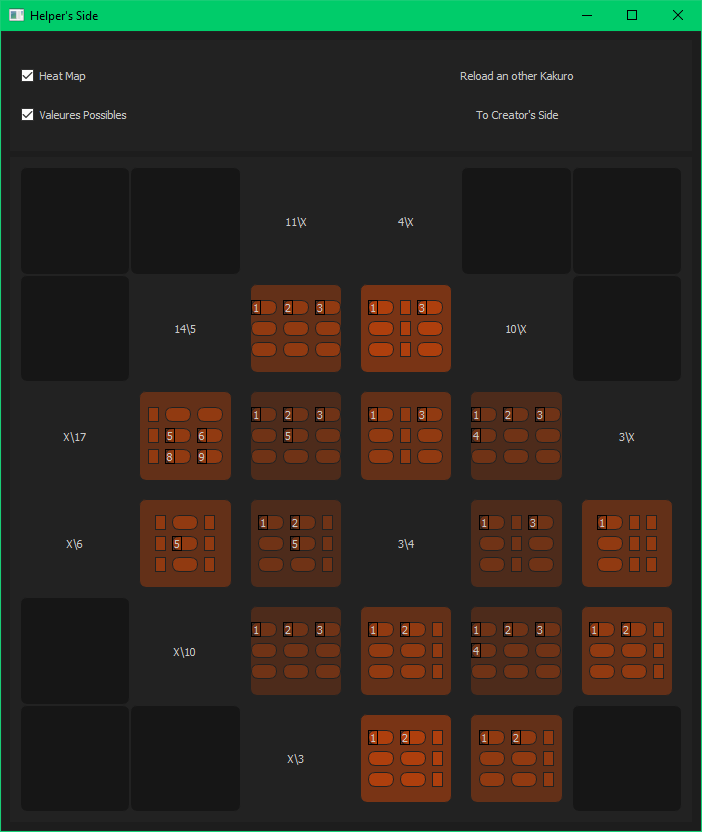
\includegraphics[width=\textwidth]{./ressources/aideMax.png} 
  \end{center}
  \caption{Il est possible de combiner la heat map et l'affichage des valeurs.}
\end{figure}

\begin{figure}[ht]
  \begin{center}
    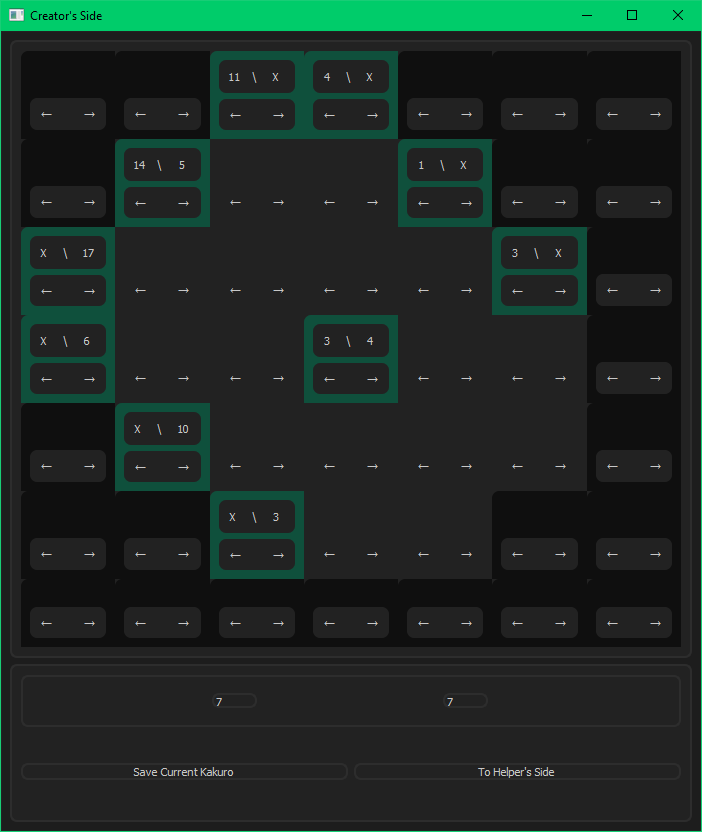
\includegraphics[width=\textwidth]{./ressources/creator.png} 
  \end{center}
  \caption{La fenêtre d'édition de grilles de Kakuro.}
\end{figure}

\end{document}

